\documentclass[bwprint]{gmcmthesis}
\usepackage[framemethod=TikZ]{mdframed}
\title{高压油管稳定控压策略的研究}
\baominghao{22103350008} %参赛队号
\schoolname{浙江大学}%学校名称
\membera{葛明阳} %队员A
\memberb{郑欣怡} %队员B
\memberc{董萌苇} %队员C
\begin{document}
\sloppy

 %生成标题
 \maketitle

 %填写摘要
\begin{abstract}
缺
\keywords{混合整数线性规划;混合整数非线性规划;粒子群算法;FFF;贪婪;BL;优先搜索;}
\end{abstract}

%\pagestyle{plain}
%目录 不推荐加
%\tableofcontents

\section{问题重述}
\subsection{问题背景}

方形件产品(也称板式类产品)是一类以板材为主要原片、经平面加工后组合装配形成的产品,如3C(计算、通讯、消费电子)、板式家具、玻璃、钣金件等。因其“多品种小批量”的个性化定制生产模式,企业通常需要进行订单组批和排样优化,降低原材料消耗,保证生产效率。

\textbf{订单组批}是指针对数量庞大的不同订单,将其组成若干批次,实现批量化生产。批次的定义为完成若干订单全部任务且不含任何不完整订单任务的订单集合。订单组批时,通常会将具有相同材质、交货期相近、工艺相似的订单安排在同一个生产批次。

\textbf{排样优化}是指合理规划方形件在板材原片上的布局,最大化材料利用率,简化切割过程。切割工艺根据是否任何一次直线切割都能保证板材可分离可分为齐头切和非齐头切,齐头切又可根据是否在有限切割阶段数内切割出准确尺寸的方形件分为精确方式和非精确方式。以3个阶段的切割方式为例,第1阶段切割生成模块可称为stripe(条带),第2阶段切割生成模块可称为stack(栈),第3阶段生成模块可称为item(产品项)。

\quad
\subsection{问题提出}
基于上述问题背景,根据题目提供的输入参数(包括单个批次产品项总数上限和面积总和上限、原片长度和宽度)和产品项数据集(包括产品项材质、数量、长度、宽度和订单号),完成下述两个问题:

\textbf{子问题1},考虑相同材质的产品项,忽略订单组批过程,在采用齐头切的三阶段精确排样方式下,给出产品项排样方法,将所有产品项排样,得到板材用量最少(即板材利用率最高)的排样方案。并利用数据集A对排样方法加以验证,将数据集A的排样结果以表格、示意图的形式进行展示描述。最后,对排样方法进行评价。

\textbf{子问题2},在问题1的基础上,解决订单组批问题。在具有不同材质、不同订单号、不同产品项大小的情况下。考虑同一订单产品项全部在同一批次、同一材质产品项方可使用同一板材原片、每个批次产品项总数和面积总和均不超过上线的约束,采用齐头切的三阶段精确排样方式,给出组批方法,得到总板材用量最少的订单组批方案及相应各批次排样方案。并利用数据集B加以验证,将数据集B的组批和排样结果以表格、示意图的形式进行展示描述,并对组批方法进行评价。

\newpage

\section{模型假设}

(1) 只考虑齐头切的切割方式(直线切割、切割方向垂直于板材一条边,并保证每次直线切割板材可分离成两块);

(2) 切割阶段数不超过3,同一个阶段切割方向相同;

(3) 排样方式为精确排样;

(4) 假定板材原片仅有一种规格且数量充足;

(5) 排样方案不用考虑锯缝宽度(即切割的缝隙宽度)影响;

(6)所有订单的交货期均相同;

(7)所有产品项的宽度均小于板材原片的宽度,高度均小于板材原片的高度。

\quad

\section{符号说明}
{\centering
\newcommand{\tabincell}[2]{\begin{tabular}{@{}#1@{}}#2\end{tabular}}
\begin{tabular}{cccc}
 \hline
  \makebox[0.05\textwidth][c]{序号}  &  \makebox[0.2\textwidth][c]{符号}	&  \makebox[0.65\textwidth][c]{意义} \\ \hline
  1 & $n$            & 同一数据集下的产品项总个数      \\ 
  1 & $i$            & 产品项编号($i\le n,i \in \mathbb{N}^+$)      \\ 
  1 & $j$            & 栈编号($j\le n,j \in \mathbb{N}^+$)      \\ 
  1 & $k$            & 条带编号($k\le n,k \in \mathbb{N}^+$)      \\ 
  1 & $l$            & 板材原片编号 ($l\le n,l \in \mathbb{N}^+$)     \\ 
  2 & $Item_{i}$     & 编号为$i$的产品项	  \\ 
  3 & $Stack_{j}$    & 编号为$j$的个栈       \\ 
  4 & $Stripe_{k}$   & 编号为$k$的条带	  \\ 
  5 & $Bin_{l}$      & 编号为$l$的板材原片  \\ 
  6 & $h_{i}$      & 产品项$Item_i$的高度(单位:mm) \\ 
  7 & $w_{i}$      & 产品项$Item_i$的宽度(单位:mm) \\ 
  8 & $H$          & 板材原片的高度(单位:mm)\\ 
  9 & $W$          & 板材原片的宽度(单位:mm) \\ 
  10 & $a_{j,i}$    & 标志$Stack_j$是否包含$Item_i$的0-1变量  	&\quad   \\  
  11 & $b_{k,j}$    & 标志$Stripe_k$是否包含$Stack_j$的0-1变量 	&\quad   \\  
  12 & $r_{l,k}$    & 标志$Bin_l$是否包含$Stripe_k$的0-1变量  	&\quad   \\  \hline
\end{tabular}
}
\newpage

\section{问题一排样优化}

\subsection{问题分析}

问题一解决同一批次产品项的排样优化问题,给定各产品项的长度、宽度,在满足切割规则和订单完整交付的条件下,对所有产品项进行排样,使总板材的用量尽可能少。根据假设(4),板材原件规格只有一种,即面积一定,故使总板材的用量尽可能少的目标等价于使板材原件的使用数量最少。

\textbf{三阶段2BP问题} \quad 这是一个三阶段二维装箱问题(two-dimensional bin packing,2BP),我们有一批n个矩形的产品项,它们的高度是hi和wi,i=1,...,n,目标是将它们包装成数量最小的箱子,在本问题中箱子即指板材。可行解决方案由一组板材组成,每个板材由一组条带组成,每个条带由一组堆栈组成,每个堆栈由一组宽度(或长度)相同的产品项组成。

\textbf{标准排样形式} \quad 对于某一可行解决方案,其使用板材数量及排样方案确定,任一板材中所含产品项的移动并不改变此板材的可利用面积,故不改变整体的板材使用方案及数量。为规范问题分析与求解,我们通过将每个产品项移动到板材最左边和最下面的位置,形成所谓的排样标准形式,示例见图1。在后续问题讨论中,我们只考虑标准形式排样。

\textbf{板材及各组成的编号规则} \quad 对于某一可行解决方案,其使用板材数量及排样方案确定,任一板材中所含条带的顺序改变、任一条带中堆栈的顺序改变、或任一堆栈中产品项的顺序改变,均不会改变此板材的可利用面积,故不改变整体的板材使用方案及数量。考虑实际排样场景,宽度近似的情况下,高度较长的产品项相比高度较短的产品项,对板材余料的可用性要求更高,即能找到可容纳的板材类型更少。因此优先考虑高度更长的产品项纳入板材排样,由高度小的板材作为灵活插入项,去提高已排长产品项的各板材的使用面积,理论上可一定程度上比随机选取产品项排样效率更好。故我们按照h1>=h2>=...>=hn的顺序,对产品项进行编号。一个可行解决方案最多包含n个堆栈,我们取其所含产品项的最小编号作为此堆栈的编号。在此编号规则下,对于堆栈j,我们可以知道它一定包含且所含产品项最长的是产品项j,且编号小于j的产品项均不在此堆栈中。故这样的编号规则可以给后续建模即计算带来较优的简化。类似的,约定一个解决方案最多有n个条带,用条带所含堆栈中最高堆栈对应的编号,作为此条带的编号;一个解决方案最多需要n个板材,用板材所含条带中最高条带对应的编号,作为此板材的编号。


\subsection{模型建立}

\subsubsection{决策变量}
在4.1节编号规则的约定下,我们定义标志各产品项($Item$)、栈($Stack$)、条带($Stripe$)、板材原片($Bin$)之间包含关系的决策变量如下:
\begin{equation}   %\mbox{中文}
    a_{j,i}=
    \begin{cases}
        1, \quad  & Item_i \in  Stack_j \\
        0,\quad  & Item_i  \notin  Stack_j \\
    \end{cases},\quad j=1,...,n, \quad i=j,...n  
\end{equation}

\begin{equation}
    b_{k,j}=
    \begin{cases}
        1, \quad  & Stack_j \in  Stripe_k \\
        0,\quad  & Stack_j  \notin  Stripe_k \\
    \end{cases},\quad k=1,...,n, \quad j=1,...n
\end{equation}

\begin{equation}
    r_{l,k}=
    \begin{cases}
        1, \quad  & Stripe_k \in  Bin_l \\
        0,\quad  & Stripe_k  \notin  Bin_l \\
    \end{cases},\quad l=1,...,n, \quad k=l,...n
\end{equation}

在此变量定义下,我们可以计算堆栈k的高度$H(k)$为:
\begin{equation}
    H(k)=\sum_{i=1}^{n} h_i a_{k,i}
\end{equation}


这样引入的模型约束是非线性的,不利于后续的求解。为了获得堆栈高度线性表达式,我们引入辅助变量$\delta_{l,i,j}$ ,它表征了产品项$i$对板材$l$中所有条带的高度有影响、并被包含于堆栈j中,其定义如下:
\begin{equation}
    \delta_{l,i,j}=  
    \begin{cases}
        1, \quad  & a_{j,i} r_{l,j}=1\\
        0, \quad  & a_{j,i} r_{l,j}=0
    \end{cases},\quad l=1,...,n, \quad k=l,...n
\end{equation}
即,$\delta_{l,i,j} = 1$当且仅当项目i包含在堆栈$j$中,同时堆栈$j$包含在条带$j$中(则堆栈i的高度会影响条带$j$的高度),同时条带$j$在板材$l$中。

则我们可以用线性的方式计算板材l的已使用高度:
\begin{equation}
\sum_{i=l}^{n} h_i r_{l,i}+\sum_{i=l+1}^{n} h_i \sum_{j=l}^{i-1} \delta_{l,i,j}
\end{equation}

\subsubsection{方向说明}
为了便于后续讨论,本文规定第一阶段切割方向为x方向,即切割方向垂直于高度、平行于长度的方向,如图\ref{方向说明1}、图\ref{方向说明2},与之垂直的板材原片的边的长度规定为板材原片的高度H,平行的边的长度规定为板材原片的长度D。
\begin{figure}[!htbp]
    \centering
    \begin{minipage}{0.48\linewidth}
        \centering
        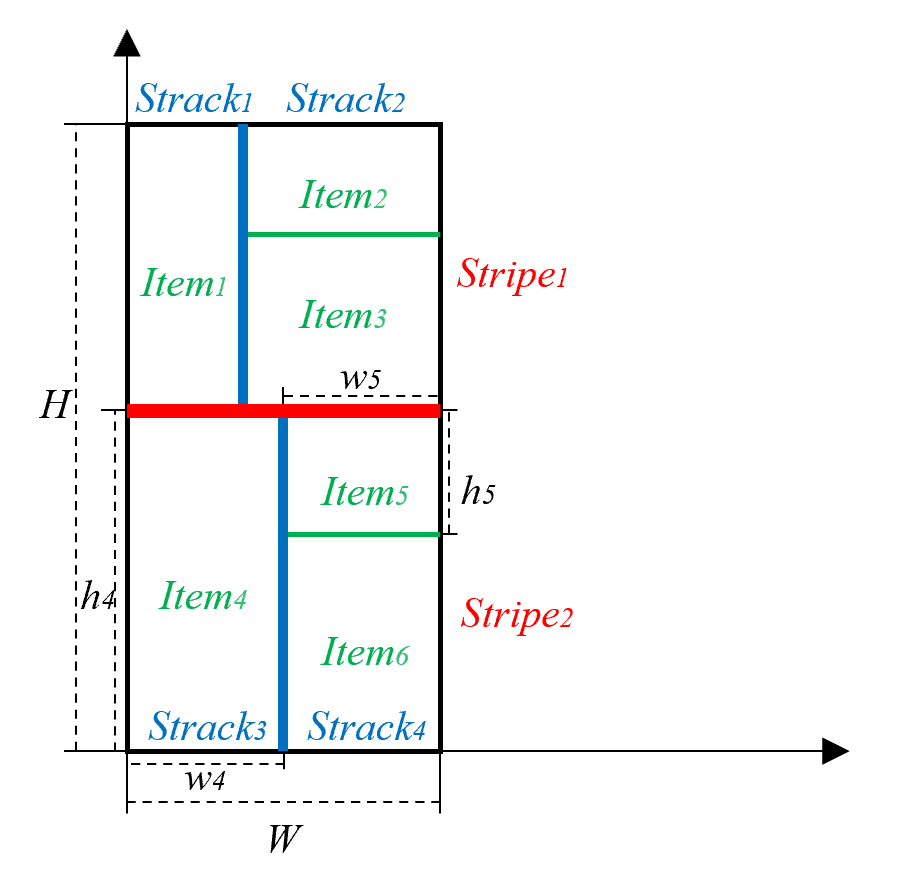
\includegraphics[width=.9\textwidth]{方向说明1.png}
        \caption{排布方案方向一}\label{方向说明1}
    \end{minipage}
    \begin{minipage}{0.48\linewidth}
        \centering
        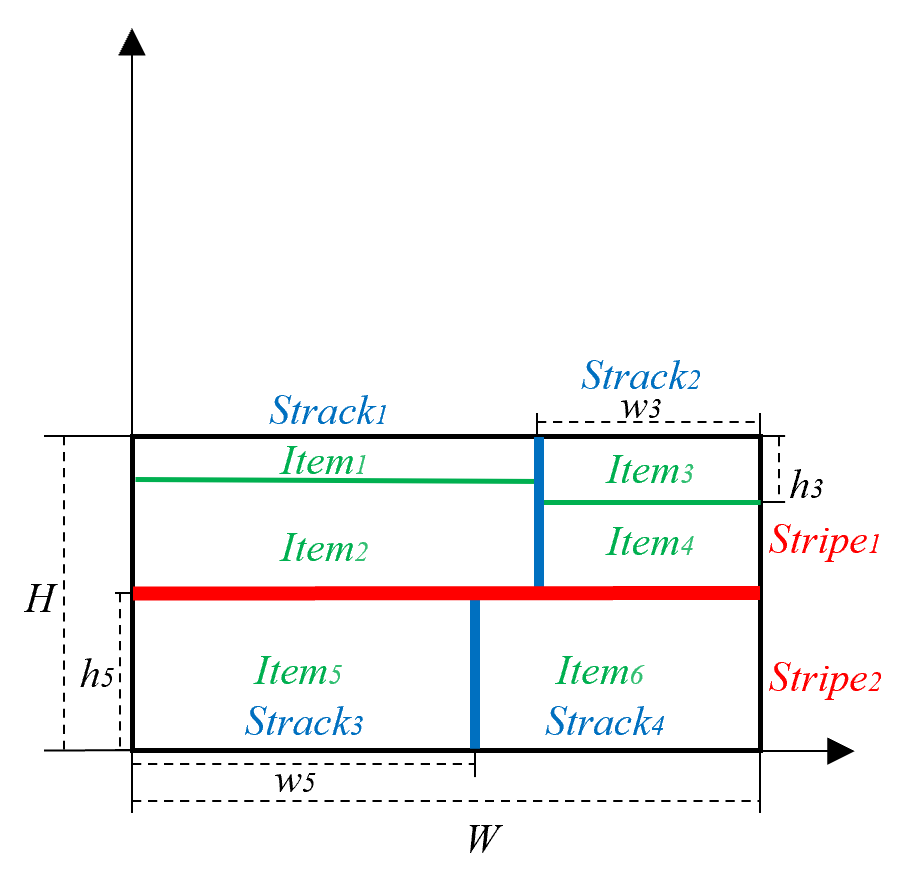
\includegraphics[width=.9\textwidth]{方向说明2.png}
        \caption{排布方案方向二}\label{方向说明2}
    \end{minipage}
\end{figure}


\subsubsection{模型建立}
%根据每次切割均必须垂直于板材边界,易知对于统一板材而言切割只有垂直于高或者垂直于宽两种方向,且各个阶段的切割方向交替进行,即第一阶段与第三阶段切割方向一致,第二阶段切割方向垂直于第一和第三阶段。为便于后续讨论,我们不妨规定在第一阶段完成尽可能多的切割。



目标函数(\ref{目标函数})是最小化所使用的板材数量,如4.1节中的问题分析,此目标与题意中的尽可能减少板材用量等价,且更为简洁直观、便于计算。当$ r_{l,l}=1 $时表示板材l被使用,故(\ref{目标函数})式即为此方案所用的板材总数。
\begin{equation}
    min \sum_{l=1}^{n}  r_{l,l} \label{目标函数}
 \end{equation}


等式约束(\label{产品项必须排})保证每个产品项i必须被排样一次。

\begin{equation}
    \sum_{j=1}^{i}  a_{j,i} =1,\quad \forall i=1,...,n \label{产品项必须排}
\end{equation}


不等式约束\label{产品项只给已使用堆栈})确保产品项只会被分配给已使用的栈$j$。
\begin{equation}
   \sum_{i=j+1}^{n}  a_{j,i} \le (n-j)a_{j,j},\quad \forall j=1,...,n-1 \label{产品项只给已使用堆栈}
\end{equation}

等式约束(19)保证了排样在同一堆栈中的产品项必须具有相同的宽度,并且任何一个堆栈中的产品项的总高度不得超过板材高度H。等式约束(20)保证每个已使用的堆栈j,被准确排样在条带j中。不等式约束(21)-(22)确保每个堆栈j的高度不会超过它所在的条带k的高度。此约束规则被拆分为“严格小于”和“小于等于”两个式子,以避免堆栈高度相同时出现歧义。等式约束(24)保证每个已使用的条带被准确打包到板材中。不等式约束(25)确保每个板材的高度大于等于所含条带的总高度。不等式约束(26)根据决策变量的定义(14)设置其值。不等式约束(27)确保没有条带被排样进未使用的板材中。

(28)-(31)为变量的范围。

完整的问题一的\textbf{三阶段2BP二进制整数线性规划模型}如下所示。

%\subsubsection{编号规则}
%
%(1)\textbf{产品项}:将各个产品项按长度从大到小排序后,从1到n依次编号;
%
%(2)\textbf{栈}:用栈中包含产品项的最小编号为该栈编号,若1到n中还有剩余编号,则这些编号分别对应一个不包含任何产品项、也不包含于任何条带的空栈;
%
%(3) \textbf{条带}:用条带中包含栈的最小编号为该条带编号,若1到n中还有剩余编号,则这些编号分别对应一个不包含任何栈、也不包含于任何板材原片的空条带;
%
%(4)\textbf{板材原片}:用板材原片中包含条带的最小编号为该板材原片编号,若1到n中还有剩余编号,则这些编号分别对应一个不包含任何条带(未使用)的空板材原片。
%
%根据上述编号规则,可知
%% (这里注意要不要写成约束)
%
%\begin{equation}
%    h_{1} \ge h_{2} \ge ... \ge h_{n}
%\end{equation} 
%\begin{equation}
%    a_{j,i}=0, \quad   j>i
%\end{equation}
%\begin{equation}
%    b_{k,j}=0, \quad   k>j
%\end{equation}
%\begin{equation}
%    r_{l,k}=0, \quad   l>k
%\end{equation}
%\begin{equation}
%    a_{j,j}=
%    \begin{cases}
%        1, \quad  & Stack_j \neq  \phi  \\
%        0,\quad  & Stack_j  =  \phi  \\
%    \end{cases}
%\end{equation}
%\begin{equation}
%    b_{k,k}=
%    \begin{cases}
%        1, \quad  & Stripe_k \neq  \phi  \\
%        0,\quad  & Stripe_k =  \phi  \\
%    \end{cases}
%\end{equation}
%\begin{equation}
%    r_{l,l}=
%    \begin{cases}
%        1, \quad  & Bin_l \neq  \phi  \\
%        0,\quad  & Bin_l = \phi  \\
%    \end{cases}
%\end{equation}
%
%\subsubsection{目标函数}
%最小化板材原片使用数量:
%\begin{equation}
%    Min \sum_{l=1}^{n} r_{l,l} 
%\end{equation}
%
%\subsubsection{约束条件}
%每个产品项当且仅当出现在一个栈中
%\begin{equation}
%    \sum_{j=1}^{n} a_{j,i}=\sum_{j=1}^{i} a_{j,i}=1
%\end{equation}  
%
%而每个非空栈当且仅当出现在一个条带中
%\begin{equation}
%    \sum_{k=1}^{n} b_{k,j}=\sum_{k=1}^{j} b_{k,j}=a_{j,j}
%\end{equation}  
%
%同理
%
%\begin{equation}
%    \sum_{l=1}^{n} r_{l,k}=\sum_{l=1}^{k} r_{l,k} =b_{k,k}
%\end{equation}  
%
%\begin{equation}
%    \sum_{i=1}^{n} r_{j,i}=1
%\end{equation}  
%
%
%\begin{equation}
%    a_{j,i}=0, \quad   h_{i}+h_{j}>H
%\end{equation}
%\begin{equation}
%    a_{j,i}=0, \quad  w_{i} \ne w_{j}
%\end{equation}
%
%
%\begin{equation}
%    a_{j,j}=1
%\end{equation}
%
%
%\begin{equation}
%    b_{k,k}=1
%\end{equation}
%
%\begin{equation}
%    r_{l,l}=1
%\end{equation}
%
%
%相同栈里的产品项宽度或长度相同
%\begin{equation}
%    \sum_{l=1}^{k} a_{l,k}=1,\quad \forall k\leqslant n
%\end{equation}  
%
%
%通过前述问题分析,我们建立了如下数学模型:
%
%\begin{equation}
%    \begin{aligned}
%    Min \sum_{l=1}^{n} r_{l,l}\\
%    Min \sum_{l=1}^{n} r_{l,l}
%    \end{aligned}
%\end{equation}  
%
%
%\begin{equation}
%    \begin{aligned}
%    Min \sum_{l=1}^{n} r_{l,l}\\
%    Min \sum_{l=1}^{n} r_{l,l}
%    \end{aligned}
%\end{equation}  



\subsection{模型求解}
	
\subsubsection{模型特点分析}
	\textbf{模型特点} 
	
	1. 变量多、呈 $ n^2 $ 量级 \quad 所建立的二进制整数线性规划模型,如式子(x)-(x)所示,其变量个数在 $ n^2 $ 数量级,约束为 n 的多项式数量级,故随着变量数量增加,求解规模将指数级增长,求解时间长甚至难以在有限步内得到解。 题目所给的数据集基本在 $ 10^4 $ 量级,由此对应的模型规模较大。
	
	2. 0-1变量、线性约束 \quad	线性规划求解发展较为成熟,但本模型的变量为0-1二进制整数类型,传统的连续线性规划、分枝定界法难以适用。
	
	\textbf{求解方向} \quad 正如4.1节的分析,问题一属于2BP问题,这是一个典型的NP-Hard问题,难以在多项式时间内求得解。有两个求解方向:一是利用传统算法例如分枝定界法、动态规划法等,在指数时间内求最优解;二是利用近似算法、近似方案或启发式算法,例如贪心算法、线性规划松弛、局部搜索、粒子群算法等,在多项式时间内求得近似解。
	
	\textbf{求解思路} \quad 结合NP-Hard可行的求解方向与本模型的特点,且经过初步的多方法求解测试,我们决定采用以下思路对问题一进行求解:设计合理简单的规则,对可行解空间进行快速贪心搜索,得到一个较优的初始解,再以此作为初值,利用启发式算法进行迭代,在多项式时间内求得近似最优解。


\subsubsection{求解算法设计}

	\textbf{1.贪心算法搜索较优初始解}
	
	


\subsection{结果分析}

\subsection{模型及算法评价}






\section{问题二订单组批}

\subsection{问题分析}

\subsection{模型建立}

\subsubsection{决策变量}

\subsubsection{编号规则}

\subsubsection{方向说明}

\subsubsection{目标函数}

\subsubsection{约束条件}

\subsubsection{数学模型}

\subsection{模型求解}
1) 对每种材质全部产品项进行排样,并按照其所需的  排序,排在前位的材质中的订单,合并在一起生产的优先级更高。

2) 

算法\ref{test}
\begin{algorithm}
    % \SetAlgoNoLine
    \caption{Put your caption here}\label{test}
    \begin{multicols}{2}
        \SetAlgoLined
        \KwData{this text}
        KwResult{how to write algorithm with \LaTeX2e }
        initialization\;
        \While{not at end of this document}{read current\;
        \eIf{understand}
        {go to next section\;current section becomes this one\;
        }{
        go back to the beginning of current section\;
        }
        }
    \end{multicols}
\end{algorithm}

\subsection{结果分析}

\subsection{结果分析}

\section{模型评价与展望}


\newpage
\quad
\newpage

%参考文献   手工录入
%\begin{thebibliography}{9}%宽度9
% \bibitem{bib:one} ....
% \bibitem{bib:two} ....
%\end{thebibliography}

%采用bibtex方案
\bibliographystyle{gmcm}
\bibliography{MCM_2022}

\cite{mittelbach_latex_2004,wright_latex3_2009,beeton_unicode_2008,vieth_experiences_2009}

\newpage
%附录
\appendix
\setcounter{page}{1} %如果需要可以自行重置页码。
\section{数据预处理及读取函数}
\lstinputlisting[language=matlab]{../code/data_pre_fun.m}
\section{问题一主程序}
\lstinputlisting[language=matlab]{../code/q1_main.m}
\section{问题一FFF算法}
\lstinputlisting[language=matlab]{../code/q1_FFF_fun.m}
\section{问题二主程序}
\lstinputlisting[language=matlab]{../code/q2_main.m}
\section{问题二XX算法}
\lstinputlisting[language=matlab]{../code/q2_tanlan.m}
\section{将计算结果保存至文件}
\lstinputlisting[language=matlab]{../code/save_to_file_fun.m}
\section{绘制排样图至文件}
\lstinputlisting[language=matlab]{../code/draw_picture_fun.m}

\end{document} 